\documentclass{article}

\usepackage[T1]{fontenc}
\usepackage[utf8]{inputenc}
\usepackage{times}

\newcommand{\autor}{Jakson Alves de Aquino}
\newcommand{\titulo}{Communication between Neovim and R}

\title{\titulo}
\author{\autor}
\date{\today}

\usepackage{tikz}

\begin{document}

\thispagestyle{empty}

\begin{figure}[htb]
    \centering
    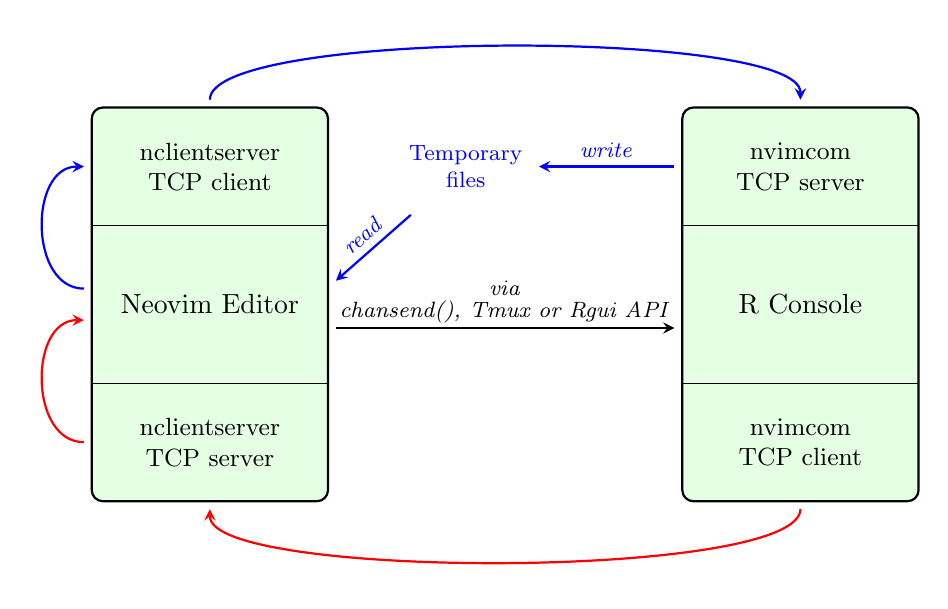
\begin{tikzpicture}[scale=1.0, >=stealth, node distance=1cm]
        \normalsize
        \draw [thick, fill=white!90!green, rounded corners] (7.5, 1.5) rectangle (10.5, 6.5);
        \draw [thick, fill=white!90!green, rounded corners] (0, 1.5) rectangle (3, 6.5);
        \node (vimed) at (1.5, 4) {Neovim Editor};
        \node (rcon) at (9, 4) {R Console};
        \small
        \draw (0, 3) -- (3, 3);
        \draw (0, 5) -- (3, 5);
        \node (pysrv) at (1.5, 5.75) [text width=2cm, align=center] {nclientserver TCP client};
        \node (pyclt) at (1.5, 2.25) [text width=2cm, align=center] {nclientserver TCP server};

        \draw (7.5, 3) -- (10.5, 3);
        \draw (7.5, 5) -- (10.5, 5);
        \node (vcsrv) at (9, 5.75) [text width=2cm, align=center] {nvimcom TCP server};
        \node (vcclt) at (9, 2.25) [text width=2cm, align=center] {nvimcom TCP client};

        \footnotesize
        \draw [->, thick] (3.1, 3.7) -- (7.4, 3.7);
        \node at (5.25, 4.2) {\emph{via}};
        \node at (5.25, 3.9) {\emph{chansend(), Tmux or Rgui API}};
        \draw [<-, thick, red] (-0.1, 3.8) .. controls (-0.8, 3.8) and (-0.8, 2.25) .. (-0.1, 2.25);
        \draw [<-, thick, blue] (-0.1, 5.75) .. controls (-0.8, 5.75) and (-0.8, 4.2) .. (-0.1, 4.2);
        \draw [<-, thick, blue] (9, 6.6) .. controls (9, 7.5) and (1.5, 7.5) .. (1.5, 6.6);
        \draw [<-, thick, red] (1.5, 1.4) .. controls (1.5, 0.5) and (9, 0.5) .. (9, 1.4);

        \node [shape=circle, text width=1.5cm, align=center, blue] (tmpf) at (4.75, 5.75) {Temporary files};
        \draw [->, thick, blue] (7.4, 5.75) -- (tmpf) node[above, midway] {\emph{write}};
        \draw [->, thick, blue] (tmpf) -- (3.1, 4.3) node[above, sloped, midway] {\emph{read}};
        \normalsize
    \end{tikzpicture}
    \caption{Communication between Neovim and R}
    \label{fig:neovim}
\end{figure}


\end{document}
